\chapter{A Medical Case Study}\label{c:medical-study}

In this thesis we primarly focus to analyze medical data by using some of the afforiomentioned techniques from section \ref{c:preliminaries}.
More specifically, we have developed algorithms for secure data aggregation and classification under the secure multi-party computation scenario.
In such a case, the computing nodes are not necessarily the ones that also provide the data.
Indeed, in our study, the data providers are hospitals and the computing nodes are three different servers.
When the medical data are transfered from the hospitals to the computing nodes, a secret sharing scheme is applied; thus it is impossible for any of the three nodes to decrypt them, and in general to infer any information.
As we examined in section \ref{s:smpc}, the only requirement of the three computing parties is not to collude simultaneously.
An ideal way to prevent collusion, is to deploy them in premises with conflicting interests.


After gathering the patients' data, the computing nodes can evaluate any arbitrary function that is deployed with respect to the SMPC model.
Any third party or analyst, can query the cluster of nodes and request a computation.


\section{Our architecture \fixme{give a fancy name for the whole scheme.}}\label{s:architecture}
Our architecture consists of the SMPC cluster and a server \fixme{find a name for that server!!} that handles all private computation requests, as well as \texttt{N} more servers that are hosted in the data providers' premises (in our case the hospitals).


The detailed procedure is depicted in figure \ref{f:overview}.
First, an analyst sends a request to the main server asking for a private computation, specifying an attribute and the hospitals from which the data will originate -- let us assume an aggregation over a field \texttt{X}, for hospitals \texttt{A} and \texttt{B}.
Then, the server request from each selected hospital to import their data for attribute \texttt{X} to the SMPC cluster.
Consecutively, using an additive secret sharing protocol, the hospitals' servers securely import their data to the three computing nodes.
The actual computation takes place after the import is complete, and finally the aggregation over attribute \texttt{X} is returned to the user through the server.



\begin{figure}[th] 
  \centering
  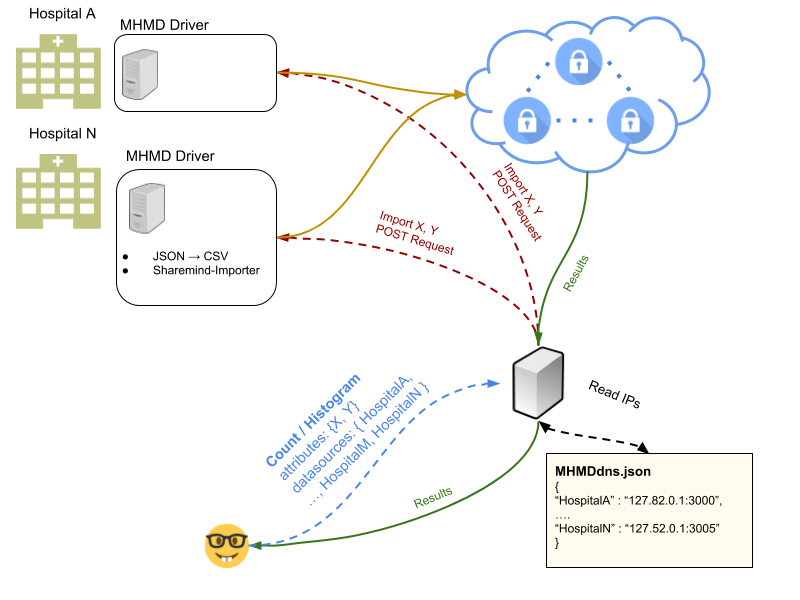
\includegraphics[width=\linewidth]{figures/overview.png}
  % \vspace{-0.2in}
  \caption{An overview of the architecture of our study}\label{f:overview}
\end{figure} 



\section{Supported Computations}\label{s:computations}
\fixme{General description of hist, id3. Details in \ref{c:pp-algorithms}
}

\fixme{what is a histogram/count and why it is usefull?}

\fixme{what is a classification tree and why it is usefull?}



